\documentclass[12pt,a4paper,twopage]{report}

\usepackage{graphicx,color}
\usepackage{subfigure}
\usepackage{amsmath}
\usepackage{amsfonts}
\usepackage{amssymb}
\usepackage{listings}
\usepackage{xspace}
\usepackage{paralist}
\usepackage{array}
\usepackage{booktabs}
\usepackage{mdframed}
\usepackage{pgfplots}

% Typesetting for units.
\usepackage[binary-units]{siunitx}

% For verbatim text with command support.
\usepackage{alltt}

% Allows multiple titles.
\usepackage{titling}

% For displaying directory trees.
\usepackage{dirtree}

% Needed to rename {algorithm} wrapped {algorithmic} sections.
\usepackage{float}

% Used for theorem formatting.
\usepackage{amsthm}

% Graphs & figures.
\usepackage{tikz}
\usetikzlibrary{arrows,backgrounds,snakes}

% Line spacing
\usepackage{setspace}

\usepackage[numbers, sort&compress]{natbib}

% hyperref redefines a number of macros, so it should be last.  Empirically,
% doing so eliminates compiler warnings.
\usepackage[bookmarks, colorlinks]{hyperref}
% According to the hyperref readme, algorithm must follow hyperref

\usepackage{algorithm}
\usepackage[noend]{algpseudocode}
\usepackage{varwidth}

%~~~~~~~~~~~~~~~~~~~~~~~~~~~~~~~~~~~~~~~~~~~~~~~~~~~~~~~~~~~~~~~~~~~~~~~~~~~~~~
% Macros

% English
\newcommand{\cf}{\hbox{\emph{cf.}}\xspace}
\newcommand{\deletia}{\ldots [deletia] \ldots}
\newcommand{\etal}{\hbox{\emph{et al.}}\xspace}
\newcommand{\eg}{\hbox{\emph{e.g.}}\xspace}
\newcommand{\ie}{\hbox{\emph{i.e.}}\xspace}
\newcommand{\scil}{\hbox{\emph{sc.}}\xspace} %scilicet: it is permitted to know
\newcommand{\st}{\hbox{\emph{s.t.}}\xspace}
\newcommand{\wrt}{\hbox{\emph{w.r.t.}}\xspace}
\newcommand{\etc}{\hbox{\emph{etc.}}\xspace}
\newcommand{\viz}{\hbox{\emph{viz.}}\xspace} %videlicet: it is permitted to see
\newcommand{\vs}{\hbox{\emph{vs.}}\xspace}

\newcommand{\todo}[1]{{\color{red}(TODO: #1)}}
\newcommand{\eb}[1]{\todo{Earl: #1}}
\newcommand{\mc}[1]{\todo{Morrison: #1}}

%% Heisentest Terms
\newcommand{\ourtitle}{Smashing Heisentests}

\newcommand{\venera}{\emph{Venera}\xspace}
\newcommand{\venerainst}{\emph{Venera Instrumentation}\xspace}
\newcommand{\heisentest}{\emph{Heisentest} \venera}
\newcommand{\flaky}{flaky\xspace}
\newcommand{\Flaky}{Flaky\xspace}
\newcommand{\Flakiness}{Flakiness\xspace}
\newcommand{\flakiness}{flakiness\xspace}

\newcommand\bench[1]{\textsf{\small #1}}

% Maths operators
\DeclareMathOperator*{\eq}{=}

%% Document-specific hyperref options
\hypersetup{
pdftitle={\ourtitle},
    pdfauthor={Earl T. Barr and Morrison Cole},
    plainpages=false,
    linkcolor=blue, % Overriding these colors to black is somewhat unfortunate
    %citecolor=black, % b/c the defaults are useful in color.
    citecolor=blue, % b/c the defaults are useful in color.
    filecolor=black,
    urlcolor=blue
}
\def\sectionautorefname{Section}
\def\subsectionautorefname{Section}
\def\subsubsectionautorefname{Section}
\newcommand{\subfigureautorefname}{\figureautorefname} %for subfigures
\newcommand{\defref}[1]{\hyperref[#1]{Definition~\ref*{#1}}}
\renewcommand{\algref}[1]{\hyperref[#1]{Algorithm~\ref*{#1}}}
\newcommand{\lineref}[1]{\hyperref[#1]{Line~\ref*{#1}}}

% Paragraph formatting
% \setlength{\parskip}{\baselineskip}
% \setlength{\parindent}{15pt}

% Line spacing
\onehalfspacing

\pagestyle{plain}
\pagenumbering{arabic}

%% lstlisting
\lstset{
	basicstyle=\ttfamily\small,
	numbers=left,
	language=Java,
	captionpos=b,
	breaklines=true,
	escapeinside={(*@}{@*)},
	breakatwhitespace=true,
}

\makeatletter
\newcommand*\SuppressNumber{%
	\lst@AddToHook{OnNewLine}{%
		\let\origthelstnumber\thelstnumber%
    	\let\thelstnumber\relax%
    	\advance\c@lstnumber-\@ne\relax%
    }%
}

\newcommand*\ReactivateNumber{%
	\lst@AddToHook{OnNewLine}{%
   		\let\thelstnumber\origthelstnumber%
   		\advance\c@lstnumber\@ne\relax%
	}%
}
\makeatother

% Algorithms
\algrenewcommand\algorithmicrequire{\textbf{Input:}}

% For theorems
\theoremstyle{definition}
\newtheorem{defn}{Definition}[section]

\begin{document}

\label{sec:title}

\begin{titlepage}
\begin{center}

{\huge \bfseries Smashing Heisentests \\[3cm]}

\textsc{\LARGE Morrison Cole}\\[0.5cm]
\textsc{\large BSc Computer Science}\\[0.3cm]
\textsc{\large Submission date: May 2, 2014}\\[2cm]

\textsc{\LARGE Supervisor: Earl Barr}\\[0.5cm]

\vfill

{\itshape This report is submitted as part requirement for the BSc Degree in Computer Science at UCL. It is substantially the result of my own work except where explicitly indicated in the text. The report may be freely copied and distributed provided the source is explicitly acknowledged.}

\end{center}
\end{titlepage}


\label{sec:abstract}

% No more than half a page and typically consists of three short paragraphs.
\begin{abstract}

\begin{framed}
	\begin{itemize}
		\item What the project is about, the principle aims and goals, and specific challenges.
		\item How you carried out the project and what work it involved.
		\item The results and achievements of the project.
	\end{itemize}
\end{framed}

\end{abstract}


%% Contents. Perhaps use figures / tables.

% Force top-level sections to enumerate with natural numbers even on the
% 'report' type document.
\renewcommand\thesection{\arabic{section}}

\tableofcontents
\newpage
%\listoffigures
%\listoftables

% Makes all pages the height of the text on the page. No extra vertical space is
% added.
\raggedbottom

\noindent``\textit{Left uncontrolled, non-deterministic tests can completely
destroy the value of an automated regression suite.}''

\hfill Martin Fowler

\section{Introduction}
\label{sec:intro}

Software is ubiquitous. With applications targeting a diverse set of
environments and platforms, developers commonly turn to automated testing with
the hope of preventing defects. Tests exercise a program over its input domain
to validate its functionality on that input or fail. Ideally, tests are
deterministic: they either always pass or always fail. In the case of regression
testing, each test allows a developer to make changes --- functional or
otherwise --- to the code under test with the confidence that existing behaviour
will not be modified. During feature development, tests have a similar benefit.
A passing test confirms that a new feature is behaving correctly. Test suites
are run regularly as part of the development cycle; unintended behaviour is
brought to the developer's attention by one or more failing tests. Despite their
benefits, automated tests are ultimately just more software, and just as
software is rarely bug free, automated tests are often plagued with bugs of
their own --- they are not always deterministic.

An intermittently failing automated test that fails often enough can be made
effectively deterministic with iteration so long as it is cheap. We call those
that are expensive or rarely fail \emph{flaky} tests.

Environmental factors are often related to intermittent test failure. The
further we travel up the layers of the pyramid, the more environmental factors
we introduce. Unit tests target and exercise isolated sections of code. A well
written unit test's outcome is almost guaranteed to depend only on the behaviour
of the code it exercises. Integration tests may depend on an external service
(\eg, a database), so may sometimes fail unexpectedly. Most vulnerable are
acceptance tests. Since they run on a complete system, they are potentially open
to interference by any number of environmental events or characteristics. For
example, an operating system starved of memory could kill the application, or, a
particularly slow start-up time could cause a timeout to occur.

\subsection{\Flaky Tests are a Real Problem}

\Flaky tests are no small issue. Mozilla\cite{mozillaFlakyTestBug} and Chromium
have known flaky tests. Android even includes an {\tt @FlakyTest}
annotation\cite{androidFlakyInterface} in its testing kit for automatic re-
running of known \flaky tests. The {\tt @FlakyTest} Android annotation has been
present since the initial release of Android.

When the latest changes are due to be released, the \flaky tests must be
considered. Normally, a particular software iteration would be held back until
all tests pass, but with \flaky tests thrown into the mix - it may take multiple
runs before all the tests pass at once - again, adding overhead.

The set of \flaky tests causes confusion, obscures real failures and erodes
trust.

Simply surpressing the \flaky tests is not a long-term solution. Informally, let
a valid test be a test that asserts that some unit of the application behaves as
expected. A redundant test might check behaviour that is not required, or is
tested thoroughly elsewhere. Assuming all tests in a suite are valid, then any
\flaky tests in the suite are also valid. A \flaky test may cover behaviour that
is not tested elsewhere. Suppressing (temporarily retiring) the \flaky test may
do more harm than good, since the behaviour it previously tested will now be go
completely unchecked unless manually tested upon each commit.

\subsection{Automating the Diagnostic Process}

Our goal is to automate as much of the process for fixing a flaky test as
possible, freeing developers to spend time developing the software, rather than
debugging tests that are in fact intended to speed up the development process.
Ultimately, each test case must be investigated and fixed by a developer, but as
we will show, much of the legwork can be automated.

The tool we propose --- \textit{\venera} --- gathers and analyses information
much in the same way as a developer would. First, it identifies the flaky tests
in a test suite. Then, it employs techniques similar to those discussed by
\citet{ArumugaNainar:2010:ABI:1806799.1806839} to gather relevant debugging
information over a series of test runs. Finally we analyze the gathered data and
identify predicates strongly associated with test failure. Our tool takes
advantage of the continuous integration environment, gathering data each time an
associated test suite is run. Figure \ref{fig:developer_workflow} shows a high-
level \venera workflow.

Previous and potential future work with an industry software startup lead us to
target the Android platform for our proof of concept.

\begin{figure}[h]

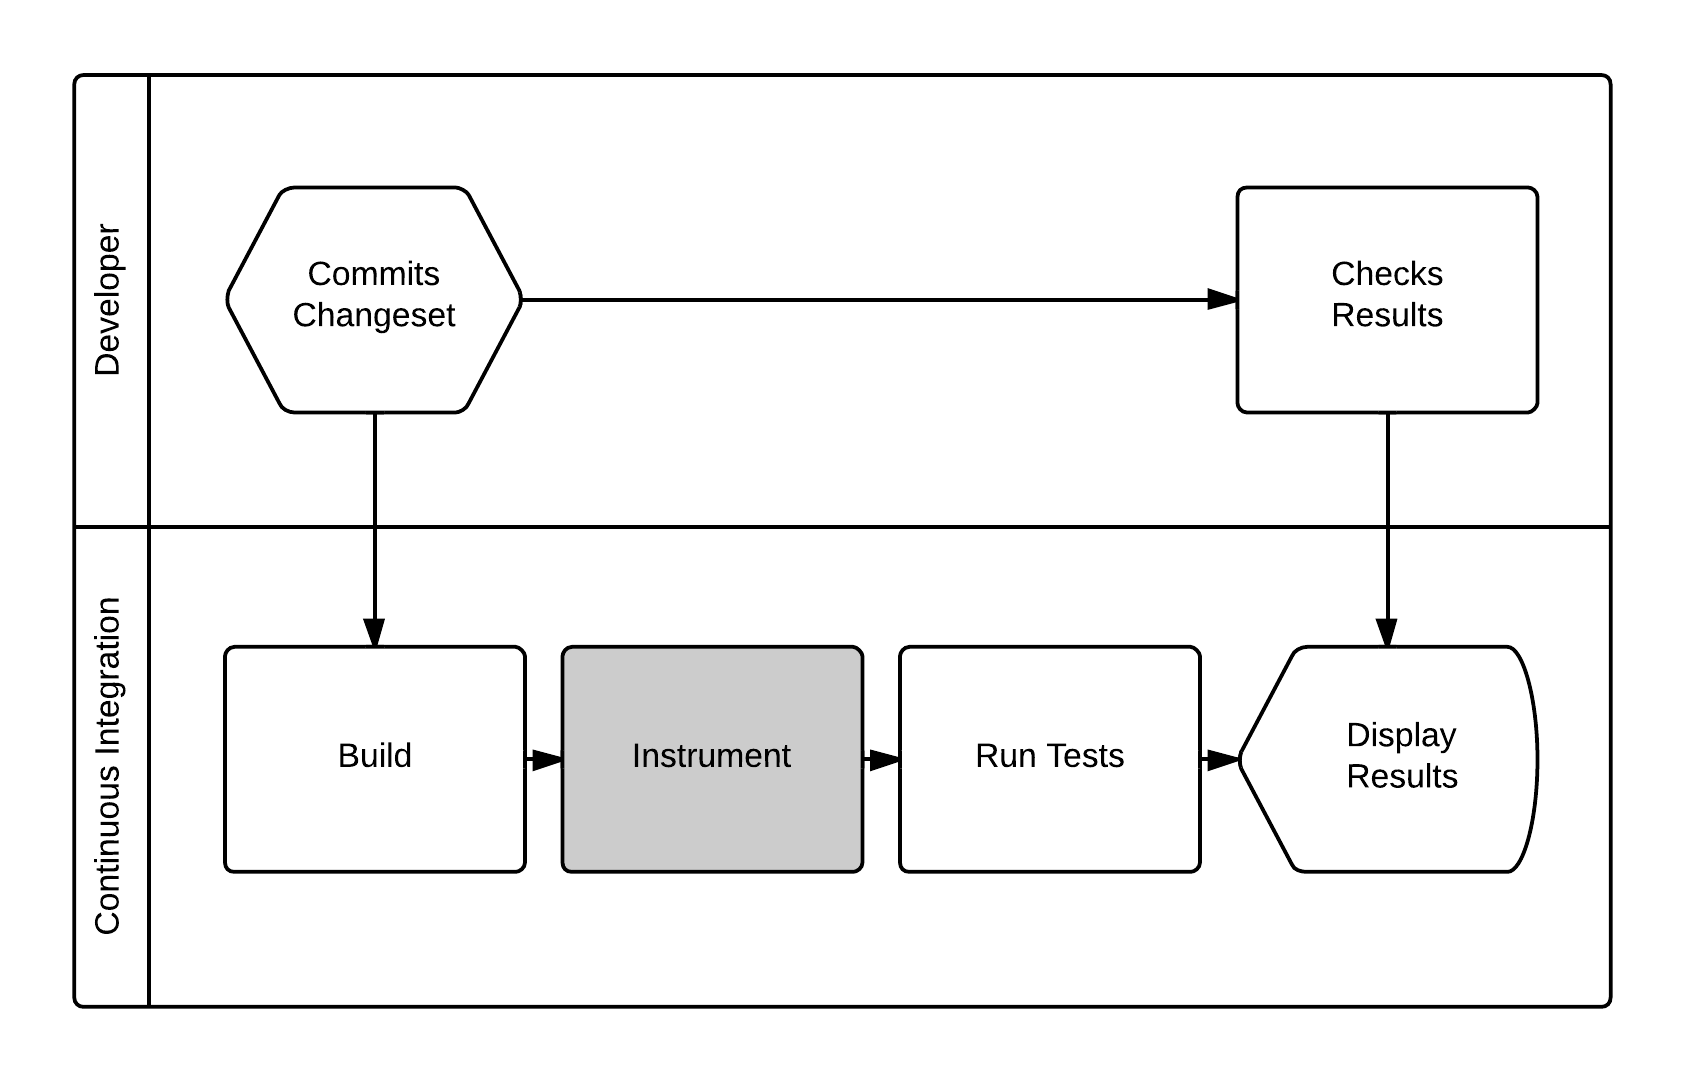
\includegraphics[width=\linewidth]{Images/developer_workflow}

\caption{}
\label{fig:developer_workflow}
\end{figure}

Running as a continuous integration step is a natural application. For one, test
suites are run as continuous integration steps themselves. In addition, we want
to be as transparent as possible.

One of the primary initial goals of the project was to create a continuous
integration plugin to present the data gathered during the identification of the
\flaky tests. As we researched the area, we realised that the indentification of
\flaky tests is the most well-covered and least interesting area. The more
experimental and relatively untouched area dealing with adaptive instrumentation
and analysis of collected information eventually became our primary focus.

Reaching a stage where we could analyze the gathered data proved to be far more
challenging than expected. The relative youth of the Android platform was a
clear stumbling block, since tried and tested instrumentation tools in the world
of the Java Virtual Machine had only just begun to acknowledge their Dalvik
sibling. As such, we document and discuss many of our design decisions along the
way.

\Flaky tests are hard to reproduce. In general, there are three stages during
which we may intervene:
\begin{enumerate}
	\item Identification - which tests in the suite are flaky?
	\item Prioritisation - which of the \flaky tests should we fix first?
	\item Resolution - what information can we gather to speed the resolution of a test?
\end{enumerate}

Ultimately, the final stage is the target. In order to tackle the problem
practically, knowledge gathered at each stage must be combined and considered.

Existing tools provide answers to 1. This information can be used to inform
manual inspection of 2. As of yet, no tool exists to tackle 3.

In a typical software development project, continuous integration systems will
be set up from the beginning. Developers write code and commit to source
control. A master server will detect the change and assign one of a number of
build agents (other servers with the capability to build the project(s) -
virtual or otherwise) an attached job.

For a typical job, the chosen build agent pulls down the latest changes,
compiles and runs the tests and runs any post-build tasks. At the end, any build
artifacts (distributable packages, test results, etc.) will be uploaded to the
master server and the agent will be once again free to build the next iteration.
Note that in reality, a job can comprise of any number of runnable steps - from
executing a shell script to hitting an external server.

It is obvious that, if we are to develop a tool to assist developers with \flaky
tests, we should run as part of a modular continuous integration system.

The rest of the report will proceed with a familiar structure.
\autoref{sec:context} describes the theory and context behind the project.
\autoref{sec:example} presents a motivating example of a \flaky test. Following
the example, we detail our general approach in \autoref{sec:approach}.
\autoref{sec:imp} discusses the design and of our proof of concept tool,
\venera. Finally, \autoref{sec:relwork} compares our work to that of previous
research and tools. We wrap up with a conclusion (\autoref{sec:conc}) and
suggest future directions for both \venera and the research in general.

\section{Context}
\label{sec:context}

\mc{This section will cover any formalisms that are necessary to understand and
model the problem.}


\subsection{\Flaky Tests}
\label{sec:sec:flaky_tests}

A test consists of a set of inputs and a corresponding expected output, over
some subject under test. In a perfect world, a test always produces the expected
output provided the subject's behaviour is fixed. In reality, environmental and
chance factors can affect the actual output. We can model the expected output
probabilistically.

\begin{quote}
	A \flaky test is one known to fail with low probability.
\end{quote}

\begin{defn}[\Flaky Test]
\label{def:flaky_test}

Let $\vec{I}$ be the lifting of all inputs, including coin flips and
environmental interactions, into a single input vector. $\vec{O}$ is the
corresponding desired output. Given a subject under test $f: \vec{I} \rightarrow
\vec{O}$, a test case is $(\vec{i},\vec{o})$. A \emph{\flaky test case} is one
where
%
\begin{align*}
  p(f(\vec{i}) \ne \vec{o}) = \epsilon
\end{align*}
%
for non-negligible probability $\epsilon \in (0..\alpha]$.

\end{defn}

Flaky tests fail rarely.  What is {\lq}rare{\rq} depends on the problem and the
cost of the test.  If a test fails frequently enough, it can be converted into a
standard failing test by repeatedly running the test, subject to the cost of
that test.  The parameter $\alpha$ represents this threshold between
reproducible via repetition and not.  The exact probability $\epsilon$ must be
non-negligible so that repeated trials are likely to trigger the failure.  In
practice, this constraint is easily met, since it is hard to imagine that a
negligible $\epsilon$ matters.  Combined with our budget $B$, we can determine
what values of $\epsilon$ we can afford to detect. \mc{We have make this
connection explicit:  maybe not here in this report, but certainly for ICSE.}

Figure~\ref{fig:flakiness} depicts \flaky tests in terms of probability of
failure.

\begin{figure}[h]
\begin{center}
	% See: http://www.texample.net/tikz/examples/line-plot-example/
	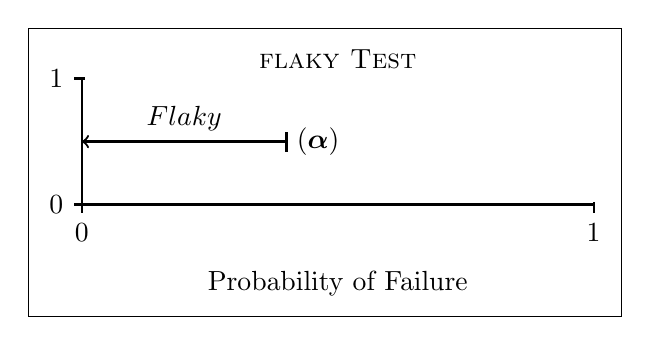
\begin{tikzpicture}[thick, framed, x=6.5cm, y=1.6cm]
		% Title
		\draw (0.5, 1) node[above] {$\textsc{\flaky Test}$};

		% Axis
		\draw (0,0) -- coordinate (x axis mid) (1,0);
	    \draw (0,0) -- coordinate (y axis mid) (0,1);

	    % Axis Labels
	    \node (padding) [below] at (0.4, 0) {};
		\node[below of = padding] at (x axis mid) {Probability of Failure};

	    % Ticks
	    \foreach \x in {0, 1}
	    	\draw (\x, 1pt) -- (\x, -3pt) node[anchor=north] {\x};
	    \foreach \y in {0, 1}
	    	\draw (1pt, \y) -- (-3pt, \y) node[anchor=east] {\y};

		% \flaky test range
	    \draw[<-] (0, 0.5) -- (0.4, 0.5); % Draw horizontal line
	    \draw (0.4, 0.42) -- (0.4, 0.58); % Draw right vertical tab

	    % Flakiness label
	    \node [above] at (0.2, 0.5) {$Flaky$};

	    % Alpha label
	    \node [right] at (0.4, 0.5) {$(\boldsymbol{\alpha})$};
	\end{tikzpicture}
\end{center}
\caption{}
\label{fig:flakiness}
\end{figure}


\subsection{Automated Testing}
\label{sec:sec:automated_testing}

Software development can be modelled as a cost optimisation problem: product
quality, delivery time and budget are just some of the common overarching
concerns.

Automated testing has been adopted by developers globally, from those working in
start ups to those in major corporations. As the number of environments
deployments are expected to run in increases, testing all possible variants
quickly becomes unworkable. It is impractical to manually test an application
across hundreds of devices every time it is modified.

Automated tests serve a simple purpose --- ensure the software under test
behaves as expected.

A good test suite achieves this by exercising discrete chunks of the program's
code to ensure it behaves in some expected way. At a high level, each test can
be broken into three steps - arrangement, action and assertion.

Anecdotally, the higher-level the behaviour being tested, the more likely a test
is to fail due to inputs unaccounted for. Tests that exercise seemingly valid
code can fail unexpectedly and unpredictably.

Developers working with such tests face a dilemma --- {\lq}suppress{\rq} the
tests until they are fixed, or acknowledge them but keep them active,
potentially randomly breaking the build from time to time until they are fixed.

Since the tests exercise behaviour which is needed (and indeed, works as
intended), both solutions are workarounds until the tests can be resolved.

A set of tests displaying seemingly random failure can devalue an entire suite,
so it is of utmost importance that developers fix such issues as they arise.
The test suite is not a user-facing feature and can quickly become a cost
rather than a benefit.

A developer given the task of fixing a bug in an automated test faces a similar
set of challenges as if they were to fix a bug in the application itself.

In our experience, within the context of real software development projects
developers quickly become frustrated when dealing with \flaky tests and begin to
rely on instinct in order to stay productive. In other words, they lose
confidence in the test suite. It is essential to maintain a reliable test suite
for it to remain a beneficial part of a team's workflow.


\subsection{Why not {\lq}non-deterministic{\rq}}

Flaky tests have been referred to as {\lq}non-deterministic{\rq} by
practitioners. Whilst a flaky test may well be non-deterministic (\ie, it
behaves differently on different runs), it may also be deterministic with
respect to some unknown input. Hence, flaky seems a better choice of term.


\subsection{What is a \flaky test?}

\Flaky tests tend to occur on the system level. They do not often manifest in
unit or integration tests since these tests usually simply call a function with
some parameters and check its output against some expected value in isolation
from the system as a whole (or, in the case of integration - against some
external service).

Acceptance tests, on the other hand, target the software as a whole. Developers
of software for mobile Operating Systems employ instrumentation to simulate user
input and check for the presence of elements in the user interface. Essentially,
a test can be distilled down to:
\begin{verbatim}
  Given I am in this state (arrange)
  When I do this (act)
  Then I am in this state (assert)
\end{verbatim}

\Flaky tests are commonly caused by timing issues. The action step requires the
arrange step to have completed before it runs; there must be some kind of wait
and check mechanism to block further progress until the arrange step has
finished.

For example, consider a test run that initially enters state $S_{1}$ (arrange),
where $S_{1}$ is a vector $(x_{1},x_{2},x_{3})$. Action $A$ transforms $S_1$ to
$S_2$ --- $(x_{1},x_{2},x_{3})$. Finally, the assertion checks that the current
state is equal to $S_2$.

If each value of the vector $S_{1}$ is loaded asynchronously, the test must
check for each of the vector values to be correct before $A$ is applied. If the
test checked only the first two values, the action would complete only if the
third element happened to have loaded before the values in position 1 and 2.

In practice, with hundreds of user interface elements, these types of problems
can become quite prevalent. Often, the solutions are obvious, but sometimes
there is not enough information to solve the problem.


\subsection{Why are \flaky tests a problem?}

Consider a project with small team of developers. They write acceptance,
integration and unit tests to cover every feature they add to the software.
Their test suite $T$, is made up of tests $t_{0}, t_{1}, \dots, t_{n}$. On
average, the tests take 20 minutes to run and each developer is expected to run
the entire suite locally before pushing a new feature to the development branch.
The test suite contains a number of \flaky acceptance tests $F$ written $f_{0},
f_{1}, \dots, f_{k} \text{, where $k \leq n$}$ that the team are aware of; $F
\subseteq T$.

A developer is working on a new feature and has written an Acceptance test to
ensure it works as expected. The acceptance test passes, so the developer
prepares to push the code onto the development branch. Before doing so, the
developer must run the test suite locally to ensure the work did not break any
existing functionality. The test suite runs, but 4 of the acceptance tests ---
$t_{3}, t_{7}, t_{9} \text{ and } t_{21}$ --- fail.

The developer is sure they have seen $t_{3}, t_{7} \text{ and } t_{9}$ fail
randomly before, i.e. $t_{3}, t_{7}, t_{9} \in F$. After checking with
colleagues, they assume that $t_{21} \in F$, since it appears to be unrelated
to the area of code they have been working on. The developer pushes the code.

In this example, $t_{21}$ was not actually \flaky, but had been broken by the
developers changes. It is important to recognise that, whilst in some situations
it may be possible to run the test suite multiple times to be sure, sometimes
this is impractical. Test suites may take hours, days or even months to run in
their entirety, and may contain many \flaky tests.

After the code is pushed, a different set of tests fail on the build server:
$t_{3}, t_{7} \text{ and } t_{9}$ are now passing, but $t_{21}$ has once again
failed. In this case, it is obvious that $t_{21}$ must be investigated, so the
developer’s changeset is rolled back whilst they fix the change.

This may appear to be workable, but time was almost certainly wasted. The
developer writing the new feature only became aware that they had broken
existing functionality after the second run revealed a trend. If $t_{21}$ had
failed alone, the developer would have taken action before committing the
changeset.

When a subset of tests fail randomly each time the suite is run, it is all too
easy for developers to begin ignoring real failures if and when they do occur.


\subsection{Living with \flaky tests}

When the latest changes are due to be released, the \flaky tests must be
considered. Normally, a particular software iteration would be held back until
all tests pass, but with \flaky tests thrown into the mix - it may take multiple
runs before all the tests pass at once - again, adding overhead.

The set of \flaky tests causes confusion, obscures real failures and erodes
trust.


\subsection{Why not just {\lq}suppress{\rq} the \flaky tests?}

Informally, let a valid test be a test that asserts that some unit of the
application behaves as expected. A redundant test might check behaviour that is
not required, or is tested thoroughly elsewhere. Assuming all tests in a suite
are valid, then any \flaky tests in the suite are also valid. A \flaky test may
cover behaviour that is not tested elsewhere. Suppressing (temporarily retiring)
the \flaky test may do more harm than good, since the behaviour it previously
tested will now be go completely unchecked unless manually tested upon each
commit.


\subsection{Fixing \flaky tests --- the manual way}

Sometimes, it is not possible to fix a \flaky test from the information output
by the testrunner alone. Typically, the information includes logs, an assertion
failure message and/or a stack trace. Applications with a user interface may
also provide a number of screenshots. Often, a developer will have to manually
gather information to build up an understanding of the intended flow vs. the
actual flow on failing runs. For \flaky tests with a low failure rate, this can
be a painstaking and time-consuming process. Indeed, if the \flaky test is a
timing based issue, attaching a debugger may cause the test to pass
indefinitely.

There are many ways to fix a \flaky test. A developer relies on experience and
intuition to determine the best approach.

\subsubsection{Common causes of flakiness}

First, let us consider common causes of flakiness:
\begin{itemize}
	\item Timeouts --- issues can occur when {\lq}driving{\rq} the application
	from the outside. Often, callbacks for actions are not available, so a test
	may be forced to wait on, for example, the presence of some element in the UI.
	If the wait time expires before the element is detected, the test will fail.
	\item Memory usage --- it is not uncommon for a constrained process to run out
	of memory. Again, this could be caused by operating system priorities
	unrelated to the test itself. It's obvious \textit{when} this has happened,
	but not \textit{why}.
	\item External services --- if a third party service falls over during a test
	run that depends on it, tests may fail.
	\item Left-over state --- static state can affect the execution of a test. If
	it is not cleaned up and reset, it can cause strange behaviour. This includes
	things like external databases, configuration files \etc.
	\item \todo{Might be missing something...}
\end{itemize}

Each developer familiar with these issues may employ techniques and patterns to
avoid them. However, while bug rates may be reduced, they may never be stamped
out entirely.

\subsubsection{Identification}

\Flaky tests are often split out into a seperate suite (a practice is known as
{\lq}quarantining{\rq}), so that developers may continue to receive the benefits
of a fast feedback cycle from the stable ones. This is a reasonable approach,
although it is the first step on a slippery slope to complete test suite
erosion.

But, this is jumping ahead. First, \flaky tests must be identified. How does a
developer know if a failure was genuine (\ie, failed due to a change in
behaviour it was designed to test) or unexpected?

Manual inspection of the related changeset and failure stacktrace is often
sufficient. A change in an area of the application (seemingly) entirely
unrelated to the observed test failure may indicate that the failure was indeed
unrelated and hence, the test \flaky. But, it is imprudent to operate on this
assumption alone. The test will then need to be re-run (either as part of the
suite on CI, or in isolation by the investigating developer locally). If the
test continues to fail, the change was clearly related. If not, the test is
\flaky.

The problem with this approach is that humans have limited memory. If the \flaky
test is not fixed as soon as it is identified (or moved to a quarantine), the
test can continue to cause problems further down the line. In fact, it can be
useful to examine test failure over time --- trends in failure may stand out.

A couple of projects have tackled this preliminary step of \flaky test
identification; namely, the Chromium Flakiness
Dashboard\cite{flakinessDashboard} and various Jenkins plugins. These tools
typically run as a continuous integration step. Some simply attach a value to
each test representing its likelihood of failure during any given test run.
Others also expose statistics such as \emph{stability($N$)} (the test's chance
of failure across the previous $N$ runs), successful runs since last failure and
first known failure. The Chromium dashboard includes a graphical matrix view for
visual detection of trends, displaying tests and their binary results over time.

\subsubsection{Prioritisation}

With a host of known \flaky tests, either in quarantine or in the main test
suite, how does a developer decide which tests to fix first? There are several
obvious factors which may affect prioritisation, including:
\begin{itemize}
	\item Failure type --- multiple \flaky tests exhibiting similar problems may
	be tackled as a group. Certain failure types may be considered more critical than others.
	\item Age --- a \flaky test that has been known to be \flaky for a long period
	may be prioritised over more recent additions, or vice versa.
	\item \todo{I must be missing something here!}
\end{itemize}

In the end, it is up to the development team to prioritise the \flaky tests, if
at all. With this in mind, the most useful thing we could do is expose
information to aid the decision making process. Providing the ability to group
and sort \flaky tests by the attributes listed above would no doubt be valuable.
In fact, this was an initial goal of the paper, but it was sidelined in order to
focus on the instrumentation.

\subsubsection{Resolution}

A common approach when fixing any bug (not just a \flaky test) is to step
through the code manually with the assistance of a debugger. By examining
execution flow and program state over one or more runs, a developer can often
pinpoint the cause or a related area of code. Debugging a \flaky acceptance test
in this way is often tedious, fruitless and time-consuming. Since an acceptance
test must compile and run the entire application, average run times can be
extremely lengthy. If the test must constantly be re-run in order to see it
fail, this time quickly adds up. What's more, attaching a debugger can affect
thread interleaving, potentially obscuring previously observed flaky behaviour.

An experienced developer may simply inspect the test in question to determine
the cause. The success of this method depends on the complexity and (likely)
familiarity of the bug.


\subsection{An automatic assistant}

We know why automated tests are useful, what a \flaky test is and why they are
costly. What can we do to aid the process of resolution?

We have seen that tools exist to speed the identification of \flaky tests. Some
of these tools expose information that can be useful in prioritisation, but none
touch resolution. This is the interesting part.

As we've seen, a developer will often resort to a manual execution with the help
of a debugger, to gather information on program state with the aim of
identifying the bug (or areas related to it). We could, with the assistance of
instrumentation, gather this information ahead of time. If we knew a test to be
\flaky, we could attach instrumentation to automatically gather and save
sections of program state. Using Adaptive Bug Isolation techniques, we could
output a ranked list of strongly associated program statements.

\section{Example}
\label{sec:example}

\mc{Figure ref{fig:} shows the result for}

Looking at Shazam's \Flaky Test monitor for the last 10 nightly builds is
interesting. By manual inspection, we can identify a good \flaky test candidate.

The nightly Jenkins plan runs all tests across 7 devices. Some of these are
tablets, and some phones. All have different resolutions, hardware
specifications and api levels.

Shazam's \Flaky Test Monitor gives us a historical view of the acceptance test
results of the past 10 builds. A subset of the most frequently failing
acceptance tests are shown, split by test and device. We are able to manually
infer flakiness by inspecting each row and column in isolation.

Almost immediately, we find a classic example.

com.shazam.android.acceptancetests.musicdetails.details.GenericDetailsAdaptiveInteractiveInfoTest.testThatShareIsAbsent:

Over the past 10 builds (\#572-581), this test has been run 70 times across 7
devices. During these test runs, it has failed once. This gives us a probability
of failure of:
$$ 1 / 70 * 100 = 1.43\% $$

\subsection{Manually Debugging}

We note that the failure occured on build number 577.

Looking up the column, we see that a few other tests failed during that build on
the same device (015d3b6664601604\footnote{We can map the GUID back to a
physical device during debugging if needs be.}).

The next step would be to look at the test result page for that device and test.
Thankfully, the \Flaky Test Monitor is integrated with the test runner results,
and links us straight there.

We get a full logcat log file, and a screenshot of the device taken at the point
of failure. This is typical of an acceptance test runner. \todo{Is other
information common?}.

Inspecting the logcat \todo{What is logcat?} for the test run, we find the
stacktrace:

\begin{alltt}
java.lang.AssertionError:
Expected:  Bitmap: android.graphics.Bitmap@426bbd18
but:
at org.hamcrest.MatcherAssert.assertThat(MatcherAssert.java:20)
...\footnote{Rest of stacktrace ommitted to save space.}
\end{alltt}

At this point, we have a stacktrace and a screenshot:

\begin{itemize}
	\item The stacktrace is fairly useless at this point. What is
	\quote{Bitmap@426bbd18}?
	\item Presuming the test is named correctly
	({\lq}testThatShareIsAbsent{\rq}), the screenshot seems to be in order --- we
	can see no {\lq}Share{\rq} icon on the page.
\end{itemize}

From this point, multiple debugging routes could be taken. A developer could
chose to:

\begin{itemize}
	\item Inspect screenshots from passing runs on the same device. Perhaps an
	obvious display difference will point them in the right direction.
	\item Jump straight to the relevant code (\ie, the test source code) and read
	through to ensure no obvious points of potential failure are present.
	\item Inspect the logcat log manually, perhaps comparing it to successful runs
	on the same (or different) devices. Perhaps a giveaway log statement can be
	found that will lead to a relevant code section.
	\item \todo{\etc...}
\end{itemize}

These options are limited. What if we had been running \splatter?

\section{Approach}
\label{sec:approach}

Figure \ref{fig:architecture_overview} depicts the high-level processes of
\venera that execute when an integrated project is built. There are three
major phases:

\textbf{Analysis.} Test run history is analysed and the probability of failure
for each test is calculated.

\textbf{Instrumentation.} \venera extracts the packaged application, examines
its bytecode and injects state-monitoring probes. Probe placement is informed by
available historical data and is performed with respect to a budget. Tests
determined to be \flaky are prioritised and are more heavily instrumented.

\textbf{Testing.} The test suite is run on the instrumented application; probes
fire events which are processed and logged to files. Logs are stored in a
database along with the test results after completion.

We first define our notion of budget (Section \ref{sec:sec:budget}). Then, we
present a criteria for ranking \flaky tests (Section \ref{sec:sec:flakiness}) so
that budget may be allocated intelligently. Finally, we detail algorithms that
can be used to allocate budget to tests in a suite (Section
{\ref{sec:sec:allocating_budget}).

\begin{figure}[h]

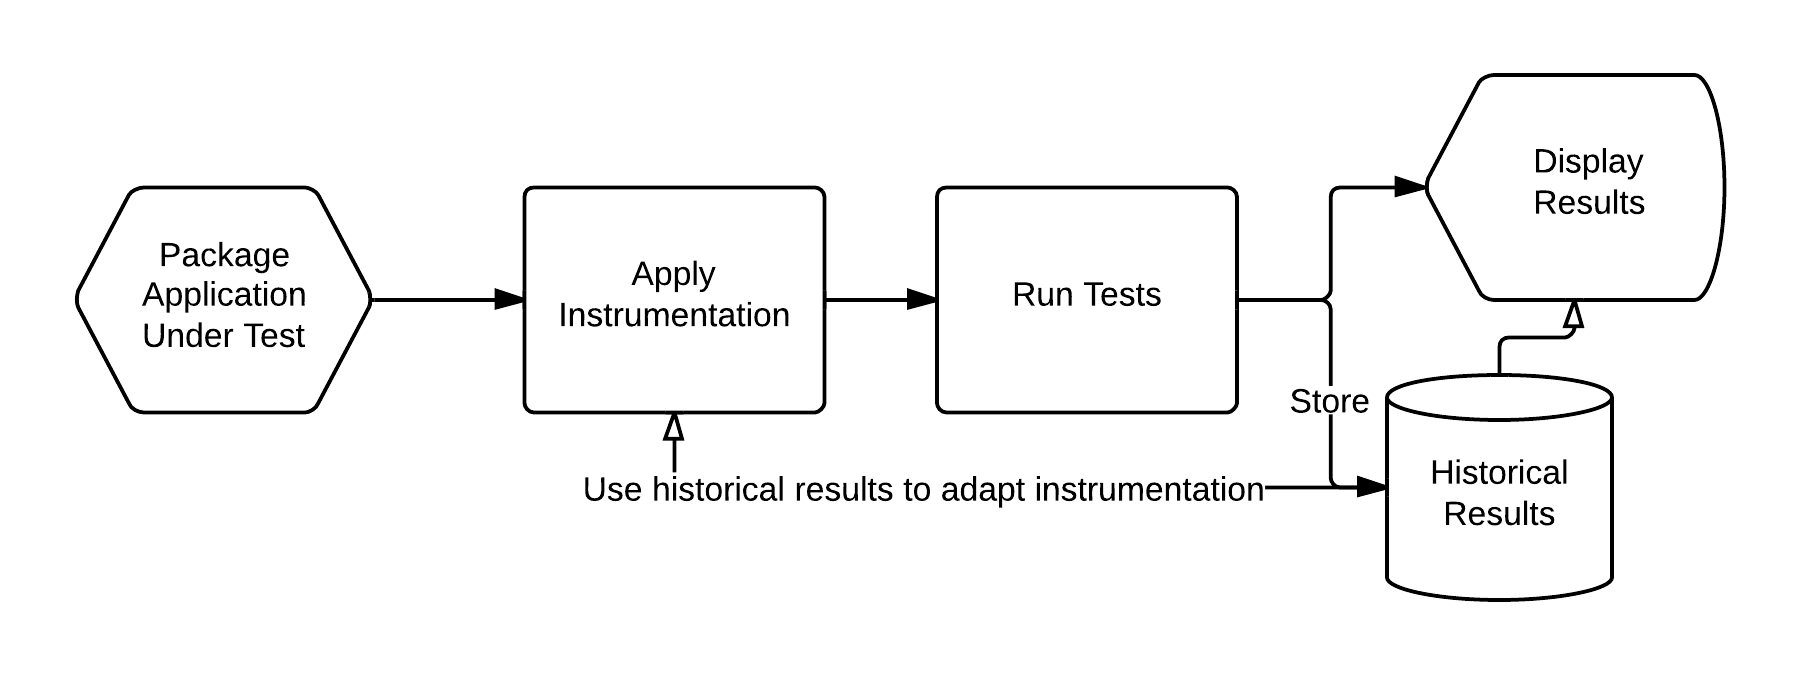
\includegraphics[width=\linewidth]{Images/architecture_overview}

\caption{}
\label{fig:architecture_overview}
\end{figure}


\subsection{Flakiness}
\label{sec:sec:flakiness}

\Flaky tests with a relatively low probability of failure are harder to
reproduce. We define a normalised scalar value --- \emph{\flakiness} (Definition
\ref{def:flakiness}) --- based on probability of test failure. We favour tests
with high \flakiness and instrument them more heavily by assigning \flaky budget
proportionally to \flakiness; Section \ref{sec:sec:allocating_budget} describes
the process in detail. Algorithm \ref{alg:calculate_flakiness} presents a
possible method of calculating \flakiness. It is important to note that
\flakiness is purely a prioritisation-related value --- we could of course
simply divide the \flaky budget equally between all \flaky tests.

\begin{defn}[\Flakiness]
\label{def:flakiness}

Given a test $T$ with probability of failure $T_{p}$, test \flakiness is
calculated by
\begin{align*}
  f(T_{p})=
	\begin{cases}
	    1 - \frac{T_{p}}{\alpha},& \text{if } T_{p}< \alpha\\
	    0,              & \text{otherwise}
	\end{cases}
\end{align*}
where $\alpha$ is the \flaky test threshold; \ie, the point at which $\epsilon$
(as defined in Definition \ref{def:flaky_test}) becomes significant.

\end{defn}

\begin{algorithm}[h]
\caption{}
\label{alg:calculate_flakiness}

\begin{algorithmic}
	\Require{$probOfFailure$ and $threshold$ are decimal values within ranges
	$[0..1]$ and $(0..1]$ respectively.}
    \Statex

	\Function{calculateFlakiness}{$probOfFailure$, $threshold$}

	\If{$(probOfFailure \geq threshold)$ OR $(probOfFailure \eq 0)$}
		\State \Return $0$
	\Else
		\State \Return $1 - (probOfFailure / threshold)$
	\EndIf

	\EndFunction
\end{algorithmic}

\end{algorithm}

\subsection{Test Suite Budget}
\label{sec:sec:budget}

Our budget is time-based. We can calculate the average time to completion for
some test suite $T$ with $\sum\limits_{t \in T} averageTimeToCompletion(t)$.
Given some maximum allowed run time $B^{max}$, we have a test suite budget $B$,
where
\begin{align*}
B = B^{max} - \sum\limits_{t \in T} averageTimeToCompletion(t)
\end{align*}

Note that a sensible value of $B^{max}$ will vary with user needs, so it will be
exposed for modification.


\subsection{Allocating Test Suite Budget}
\label{sec:sec:allocating_budget}

We partition our budget into two pools: \flaky and exploratory. Given our
total test suite budget $B$, we have
\begin{align*}
B = B_{e} + B_{f}
\end{align*}
where $B_{e}$ is the total exploratory budget and $B_{f}$ is the total flaky
test budget.

At the test level, we allocate \flaky budget proportionally to a test's
flakiness. Exploratory budget is uniformly randomly allocated over all tests ---
each test in the suite is equally likely to receive a portion of the exploratory
budget, but not guaranteed.

Given a suite of tests $T$, a test $t \in T$ is allocated budget $B_{t}$, where
\begin{align*}
B_t = \frac{B_f \times T_f}{\sum\limits_{i=1}^{|T|}
f(T_{i_p})} + \frac{B_e}{|T|} + B_{remainder}
\end{align*}
\mc{This is wrong. $B_{remainder}$ is not defined. It \textit{should} be the
remaining budget after the $B_e$ and $B_f$ are allocated. Also $\frac{B_e}{|T|}$
is not how $B_e$ is allocated --- it is allocated over all non-\flaky tests
uniformly until there is no budget remaining. In other words, not all tests will
receive exploratory budget.}

\begin{algorithm}[H]
\caption{Instrumenting the test suite with respect to a budget}
\label{alg:venera}

\begin{algorithmic}
	\Require{$T$ is the set of tests making up the test suite}
	\Require{$B$ is the test suite budget}
	\Require{$proportionFlaky$ is a decimal value in the range $[0..1]$}
	\Statex

	\Function{venera}{$T$, $proportionFlaky$}

	\Statex

	\State allocateBudget($T$, $B$, $proportionFlaky$)
	\Statex

	\ForAll {$t \in T$}
		\State{instrument($t$)}
	\EndFor

	\EndFunction

	\Statex

	\Function{allocateBudget}{$T$, $B$, $proportionFlaky$}

	\State{$flakyBudget \gets B * proportionFlaky$}
	\State{$exploratoryBudget \gets B * (1 - proportionFlaky)$}
	\Statex

	\State{allocateFlakyBudget($T$, $flakyBudget$)}
	\State{allocateExploratoryBudget($T$, $exploratoryBudget$)}

	\EndFunction
\end{algorithmic}

\end{algorithm}

\mc{$proportionFlaky$ is stupid.}

\algref{alg:venera} defines the two main steps: allocation and instrumentation.
First, $B_t$ is calculated for each $t$. Then, the instrumentation is performed.
It is during the instrumentation step that the application is actually modified.

\subsubsection{\Flaky Budget Allocation}
\label{sec:sec:flaky_budget_alloc}

\begin{algorithm}[H]
\caption{Allocating flaky budget to tests}
\label{alg:allocateFlakyBudget}

\begin{algorithmic}
	\Require{$T$ is the set of tests making up the test suite}
	\Require{$B_f$ is the total \flaky test budget}
	\Require{$B_{f}^{max}$ is the maximum \flaky budget for a test}
	\Statex

	\Function{AllocateFlakyBudget}{$T$, $B_f$, $B_{f}^{max}$}

	\State $totalFlakiness \gets 0$

	\For{$t \in T$}
		\State $totalFlakiness \gets totalFlakiness + flakiness(t)$
	\EndFor
	\Statex

	\State $T \gets$ sortByFlakinessDescending($T$)

	\For{$t \in T$}
		\State $B_t \gets$ calculateTestFlakyBudget($t$, $totalFlakiness$, $B_f$,
		$B_{f}^{max}$)
	\EndFor

	\EndFunction
	\Statex

	\Function{calculateTestFlakyBudget}{$t$, $totalFlakiness$, $B_f$,
	$B_{f}^{max}$}

	\State $testFlakyBudget \gets (flakiness(t) / totalFlakiness) * B_f$
	\Statex

	\Return minimum($testFlakyBudget$, $B_{f}^{max}$)

	\EndFunction
\end{algorithmic}

\end{algorithm}

\subsubsection{Exploratory Budget Allocation}

Exploratory budget gives us a chance of gathering data from newly flaky tests.

\begin{algorithm}[H]
\caption{Allocating exploratory budget to tests}
\label{alg:allocateExploratoryBudget}

\begin{algorithmic}[1]
	\Function{AllocateExploratoryBudget}{ $tests$, $B_e$}

	\State shuffle($tests$)
	\State $iterator \gets tests.getIterator()$
	\While{$exploratoryBudget > 0$ AND $iterator.hasNext()$}
		\State $currentTest \gets tests.getNext()$
		\State \begin{varwidth}[t]{\linewidth}
		$exploratoryBudget \gets exploratoryBudget -$\par
		\hskip\algorithmicindent \text{calculateTestExploratoryBudget}(test,
		exploratoryBudget)
		\end{varwidth}
	\EndWhile

	\EndFunction
	\Statex

	\Require{$B_{e}^{max}$ is the maximum exploratory budget for a test $t$}
	\Statex

	\Function{CalculateTestExploratoryBudget}{test, exploratoryBudget}

	\State $maximumExploratoryBudget \gets B_{e}^{max}$

	\If{$test.budget > 0$}
		\Return $0$
	\EndIf

	\State $test.budget \gets$ minimum($exploratoryBudget$,
	$maximumExploratoryBudget$)

	\State \Return $test.budget$

	\EndFunction
\end{algorithmic}

\end{algorithm}


\subsection{Instrumentation}

\algref{alg:instrument_test} details the basic process for instrumenting a test
with respect to a given budget. {\tt GetNextSetInstrumentationPoints()} returns
a list of instrumentation points ordered by descending priority. An ideal
implementation of the function would take into account previous probe
allocations, test outcomes and budgets.

\begin{algorithm}[H]
\caption{Instrument a test with respect its allocated budget}
\label{alg:instrument_test}

\begin{algorithmic}
	\Function{Instrument}{test}

	\State{$sites \gets GetNextSetInstrumentationPoints()$}
	\While{$test.budget > 0$}
		\ForAll{$site \in sites$}
			\State{$cost \gets site.cost$}
			\If{$cost \le test.budget$}
				\State{$site.active \gets true$}
				\State{$test.budget \gets budget - cost$}
			\Else
				% Need to work out how to define new algorithmic-style macros (e.g.
				% \BREAK)
				\State{\textbf{break}}
			\EndIf
		\EndFor
	\EndWhile

	\EndFunction
\end{algorithmic}

\end{algorithm}


\subsection{Prioritisation and Future Optimisations}

In the future, we could adjust \flaky budget allocation by taking into account
relative volume of historical data. For example, a newly \flaky test for which
we have little to no data may be prioritised above a known \flaky test for which
we hold a large amount of information from previous instrumented runs.

We could start from a pesimistic viewpoint. A new tests would be assumed to have
a flakiness value of 1. As the test is run, the flakiness value would be
adjusted as usual until it represented a more accurate value. New tests will
therefore be heavily instrumented, and gradually less so as they prove
themselves to be reliable.

\subsection{Monitoring Application State with Probes}
\label{sec:probes}

There are a number of types of points at which it is useful to gather
information about application state. We extend the common approach of counters
and predicates[] to include instrumentation designed for to gather much more
contextual information.

We refer to a piece of code inserted at an instrumentation site to monitor
application state as a probe. Complex probes record the state of live objects
such as variables and method parameters, but carry a large performance overhead.
Predicate probes are a lightweight alternative to monitor execution flow.

Probes are allocated based on the available budget, historical results and
available instrumentation sites. For example, predicate probes could be used to
hone in on program flows associated with failure during initial runs. Later,
once areas of problematic code are identified, heavier-weight complex probes
could then be inserted to gather more detailed information.

Complex probes serialize Java objects to JSON with google-gson. Primitives are
boxed to their object representations.

Predicate probes simply maintain a counter that is incremented each time the
predicate is observed to be true.

\begin{center}
    \begin{tabular}{| l | p{6cm} |}
    \hline
        \textbf{Program Point} & \textbf{Description} \\
    \hline
        \multicolumn{2}{|c|}{\textit{Complex Probes}} \\
    \hline
        Function Entry &
        At the beginning of each function, we serialize all parameter objects
        (boxing primitives), along with all live variables. \\
    \hline
        Function Return &
        At each function call with a return value, we serialize its object
        result. \\
    \hline
        Conditional Branch &
        At each branch point, we record all variables in scope separately for
        each path. \\
    \hline
        Variable Assignment &
        For an assignment $V = E$, where $E$ is an expression, we record both
        the current value of $V$ and the new value of $V$ after assignment. \\
    \hline
        \multicolumn{2}{|c|}{\textit{Predicate Probes}} \\
    \hline
        Conditional Branch &
        At each path of the branch we maintain a counter that is incremented
        every time the path is taken. \\
    \hline

    \end{tabular}
\end{center}

\subsubsection{Probe Cost}
\label{sec:sec:probe_cost}

In order to meet our budget, it is important that we are able to estimate the
effects individual probes have on timing. If our instrumentation causes a
individual test to run over budget, we risk running over budget at the suite
level. We refine probe costs by comparing expected overhead to measured
overhead.

To measure the effects of both the Complex and Simple Method Entry Probes, we
wrote and ran 12 tests. Each of the tests call an empty method with one or more
arguments 100 times. The tests were annotated with {\tt COMPLEX}, {\tt SIMPLE}
and {\tt NONE} policy types. The uninstrumented (\ie, {\tt NONE}) test is used
as a baseline. \autoref{lst:uninstrumented_test} shows the basic structure of
the uninstrumented test with 1 argument --- the others similar. Timings were
measured for the method calls only; start up and shutdown times were ignored.
The tests were run on a Nexus 5 running Android version 4.2.2.

\begin{lstlisting}[caption=Uninstrumented Test,label=lst:uninstrumented_test]
@Venera(instrumentationPolicy = NONE)
public void testUninstrumentedEmptyMethod() {
	Stopwatch.createStarted();
	for (int i = 0; i < 100; i++) {
		anUninstrumentedEmptyMethod(i);
	}
	Stopwatch.stop();
}

@Venera(instrumentationPolicy = NONE)
private void anUninstrumentedEmptyMethod(int unusedParameter) {
}
\end{lstlisting}

\begin{figure}[h]

\centering
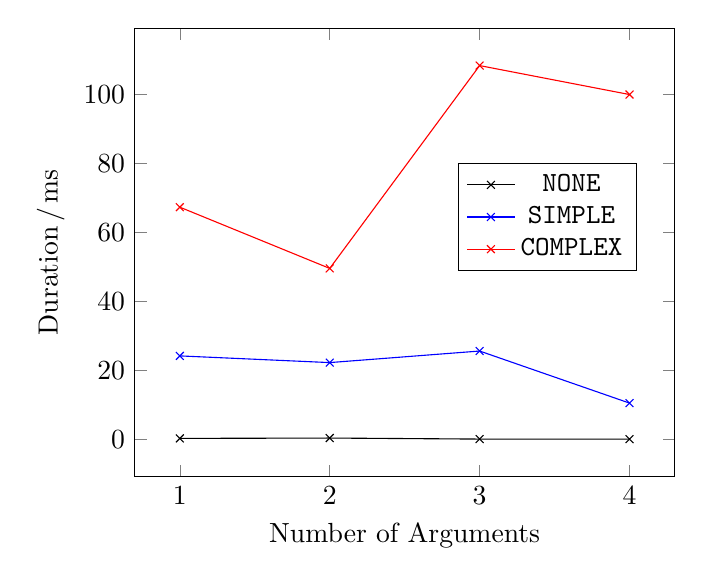
\begin{tikzpicture}
	\begin{axis}[
		xlabel = Number of Arguments,
		ylabel = Duration\,/\,ms,
		xtick={1, 2, 3, 4},
		legend style = { at = {(0.93,0.7)} },
	]
		\addplot[
			color = black,
			mark = x,
		] coordinates {
		( 1, 0.2626 )
		( 2, 0.3652 )
		( 3, 0.0645 )
		( 4, 0.0364 )
		};
		\addlegendentry{\tt NONE} ;
		\addplot[
			color = blue,
			mark = x,
		] coordinates {
		( 1, 24.17 )
		( 2, 22.23 )
		( 3, 25.58 )
		( 4, 10.49 )
		};
		\addlegendentry{\tt SIMPLE} ;
		\addplot[
			color = red,
			mark = x,
		] coordinates {
		( 1, 67.27 )
		( 2, 49.52 )
		( 3, 108.3 )
		( 4, 99.91 )
		};
		\addlegendentry{\tt COMPLEX} ;
	\end{axis}
\end{tikzpicture}

\caption{}
\label{fig:test_perf_results}
\end{figure}

With the initial results from the performance tests
(\autoref{fig:test_perf_results}), we can expect that a Complex Instance Method
Entry probe will have an associated overhead of approximately 250 times that of
the original method call, with a Simple Instance Method Entry probe having less
at roughly 60.

Our collected data is not ideal. Each of the data points is backed by only one
measured value and it is clear that the Android platform has intefered with
the results. In order to properly evaluate the cost of our probes, we will need
to measure a large number of methods over multiple runs to smooth out the data.

In the case of Complex Instance Method Entry probes, we would expect an increase
in overhead as a function of the number of parameters of the instrumented
instance method. To a certain extent, the data shows that it is indeed the case,
but it is impossible to be sure with so few data points.

\subsection{Instrumentation Points}
\label{sec:sec:instrumentation_points}

There are potentially millions of lines of code, where do we place our
instrumentation?

Given an entry point, in our case, a test or setup method, we simply take the
next set of code units in the control flow graph.

The main strategy is to place probes further and further down the control
dependence graph until we are able to detect a failure-predicting predicate.

Once we have detected a failure-predicting predicate, we can assign the majority
of our budget to drill down in related areas. Still, we reserve a portion to
‘scout’ in case we get lucky and find another failure predicting predicate
elsewhere.


\subsection{Countering the {\lq}Observer Effect{\rq}}
\label{sec:sec:observer_effect}

If our instrumentation happens to perturb the behaviour of a \flaky test in such
a way that $\epsilon$ is observed to have changed, we reduce the budget
allocated to the test until $\epsilon$ returns to its previous value.

% Focus on the interesting design decisions. For example, what were the alternatives, why select one particular solution?
% Don't flood the chapter with diagrams. Be selective.
% Avoid lengthy sections of code; use pseudo-code.
% This is a core chapter and will usually be quite substantial, 10 pages or more.
\section{Design and Implementation}
\label{sec:imp}

\begin{mdframed}
	\begin{itemize}
		\item Describe the design of what you have created.
		\item Start with the application architecture, giving its overall structure and the components that make up that structure.
		\item Give a description of the design of each of the components that make up the architecture.
		\item Include the database or storage representation.
		\item Provide implementation details as necessary.
	\end{itemize}
\end{mdframed}


This section details the design and implementation of our proof of concept tool, as it stands so far. It is comprised of two parts: a Jenkins plugin and an Android instrumentation tool.


\subsection{Jenkins Plugin}

The Jenkins plugin is a wrapper that manages the storage of the test results and associated artifacts in a HSQL database.


\subsection{Android Instrumentation Tool}

The Android instrumentation tool is a command line Java project, packaged as a \texttt{.jar}.

\subsubsection{Command Line Arguments}

It takes a number of arguments, all necessary for the correct running of the program. If any of the necessary arguments are missing, a usage message is printed and the program exits.

The following arguments are required:
\begin{itemize}
    \item \texttt{applicationApk} --- The fully qualified path to the Application APK to be instrumented.
    \item \texttt{testApk} ---The fully qualified path to the Application Test APK.
    \item \texttt{androidPlatforms} --- The fully qualified path to an \texttt{Android SDK/platforms/} folder.
\end{itemize}

An example usage, run from the directory containing the APKs to be instrumented, would look something like:

\texttt{splatter --applicationApk=android-app-debug.apk\\--testApk=android-app-debug-test.apk\\--androidPlatforms=\$ANDROID\_HOME/android-platforms}

We use the Apache commons-cli library for command line argument parsing and validation.

\subsubsection{Soot}

We looked into Soot for its ability to generate control flow graphs (CFGs). When searching for failure-predicting predicates, we will favor locations futher down the CFG when placing probes (new or moved). Section \todo{ref} describes this process in more detail.

It is possible to generate the CFG for a method using ASMDEX alone, although it is a slightly more tricky task.

In the end, although Soot was a nice tool to work with, we scrapped Soot for a few reasons:
\begin{itemize}
    \item The representation used by Soot is fairly incompatible with that of ASMDEX. Even if we could determine the CFG for a method using Soot, we'd have to somehow map the locations to our ASMDEX instrumentation sites --- a non-trivial task.
    \item The overhead of starting up Soot and analysing an APK is significant. \todo{how long}
    \item We want to avoid extra dependencies if possible.
\end{itemize}

\subsubsection{Hardcoded Strings}

There are various points in the application that have been hardcoded during development and never generalised. These are marked with \texttt{// TODO:} comments in the places they do exist. Obviously, these dependencies must be pulled up into the \texttt{Options} command line arguments, so that a user can modify them.

\subsubsection{Future Work}

The plugin will need to analyse historical test results and calculate the probability of failure for each test \todo{as discuss in section $n$}. It will also need to be extended with an interface to visualise test flakiness and related information {\todo bring in some of the information from approach here, flakiness tables \etc}. This is also related to prioritisation.


\subsection{A Choice of Continuous Integration Tools}

Jenkins \cite{Jenkins} is a popular open source continuous integration tool. Like others of its kind, it maintains a history of build results and their associated artifacts. A wealth of plugins provide support for testing frameworks such as JUnit --- displaying individual test outcomes, stack traces and assertions in a simple interface.

Although there are many open source alternatives which we could support (\eg, Hudson, from which the Jenkins project derives), many of these have significantly smaller user bases and commit activity. Mostly though, our decision to support Jenkins was motivated by Shazam's use of it across all teams.

Although the tool will be developed initially for Jenkins, it is essential to structure the plugin such that it can easily be migrated to other CI systems. At all stages of design, this must be kept in mind.


\subsection{A Solution}

\subsubsection{Identification}

This stage is fairly trivial since we can build upon the work of others.

After a test run completes, we can gather the test run results and store them in a persistent database. We can then look at the test runs over time and attach various values to each test much in the same way as the existing tools. ‘Flakiness’ - a percentage value representing a test’s likelihood to fail will be the most useful of these.
TODO: Write a list of values we hope to attach to each test. Back this up with quotes from Shazam.

\subsubsection{Prioritisation}

We can use the data gathered during the identification stage to rank the tests according to criteria. A simple output would be a descending list ordered by flakiness:

\begin{center}
    \begin{tabular}{ | l | p{5cm} |}
    \hline
    Test & Flakiness \% \\ \hline
    testVeryFlaky() & 91 \\ \hline
    testSometimesFlaky() & 33 \\ \hline
    testSignificantlyFlaky() & 2 \\ \hline
    \end{tabular}
\end{center}

Or, we could group the tests by common failure type, e.g.:

% \lstset{
% 	numbers=none,
% 	xleftmargin=3pt,
% 	numbersep=1em
% }

\begin{center}
    \begin{tabular}{| p{10cm} | l |}
    \hline
    Common Failure & \flaky{} Test Count \\ \hline
    {\begin{lstlisting}[language=Java, numbers=none]
java.lang.OutOfMemoryError
	\end{lstlisting}}
    & 4 \\ \hline
    {\begin{lstlisting}[language=Java, numbers=none]
java.lang.AssertionError:
Expected: (View visibility to be View.VISIBLE and View to have a width and a height)
but: View visibility to be View.VISIBLE View with id: class android.resources.R$id.anExampleView(1) had a visibility of View.GONE
	\end{lstlisting}}
	& 2 \\ \hline
    {\begin{lstlisting}[language=Java, numbers=none]
junit.framework.AssertionFailedError:
expected: "an_example_string"
but was: ""
	\end{lstlisting}}
	& 1 \\ \hline

    \end{tabular}
\end{center}

\flaky{} tests using the same troublesome method or similar logical flow may well fail with the same stacktrace or assertion failure. By automatically detecting this, developers could target groups of related tests and potentially fix an entire group at once.


\subsubsection{Resolution}

Using data from the identification and prioritisation stages, we can begin to develop an adaptive instrumentation to automatically gather runtime information whilst maintaining a low overhead.

\todo{Explain why we are ‘just’ targeting Android for now (Shazam, GUI testing, etc).}

Automated testing is used during development. We therefore can assume unrestricted access to debug builds.


\subsubsection{Architecture}

\todo{Need a diagram to show the architecture of the Heisentest plugin. Both an abstract overview and a detailed one (implementation with Jenkins) would be useful.}

At a high level, we essentially instrument the application under test and store the gathered data. We then analyse the gathered data, adapt the instrumentation and present useful information to the developers.

To keep the scope reasonable, we currently target Java Android applications. Of course, the approach is general, and could be applied to any number of languages and frameworks. A pure Java instrumentation would be fairly similar, and actually far less complex, for reasons that will be expanded upon later.

It is necessary to give an overview of the Android pipeline in order to understand how the tool works.

In a standard Java application, code is compiled into a ‘jar’ file - an archive commonly containing compiled ‘class’ files, resources, a manifest and certificates. A java compiler will generate one class file per type (including inner and anonymous) present in the source program. At runtime, the bytecode in these classes is executed by the Java Virtual Machine (JVM).

Android applications are typically written in Java and compiled to bytecode. However, Android runs processes on Dalvik - a Virtual Machine optimised for resource-constrained devices. The compiled bytecode is then transformed to ‘dex’ format and deployed as an ‘apk’. Similar to a standard JAR file, an Android APK is simply an archive containing the compiled assets for an Android application. Crucially, the resulting dex file contains all of the classes present in the application. The format is register-based, so modifying the transformed code can be tricky.

% \todo{http://davidehringer.com/software/android/The_Dalvik_Virtual_Machine.pdf}

For the purposes of the instrumentation, many of the included files can be ignored. Figure 1. shows a simplified APK with the sections that are relevant to the tool:

\dirtree{%
.1 application.apk.
.2 META-INF\DTcomment{Directory containing certificates}.
.2 AndroidManifest.xml\DTcomment{Basic info - version, name, etc.}.
.2 classes.dex\DTcomment{Dalvik-readable compiled classes; register-based format}.
}

\subsubsection{Registers}
Frames are fixed size. This means that total registers are known ahead of time (build in to the format). Space for extra information is also included (program counter etc.) but is not of consequence to us.

Arguments of a method take the final registers of the method's invocation frame. Instance methods have a \textit{this} reference passed as the first argument; the formal arguments (if any) take up the next registers in order.

For the method:

\todo{example tiny instance method with arguments}

The corresponding registers will be allocated:

\todo{colour coded register allocation (Dalvik bytecode)}

\todo{Need to detail our register allocating visitor and explain how it works / when it (might?) fail!}

\subsection{Notes}

\subsubsection{SDK}

An SDK project can (optionally) be included. It defines the annotation @SplatterIgnore. During the isntrumentation phase, if a method is found with this annotation, it is blacklisted from the list of possible instrumentation sites. This could be useful by developers during debugging, or to remove instrumentation from sites that are known to be problematic or, alternatively, {\lq}bug-free{\rq}!

\subsubsection{Instrumentation Points}
On the first pass we look at the whole application.

\textbf{Methods}
For methods that are not blacklisted or ignored due to annotations, we store the method name and owner class (\todo{should also keep track of signature / return type?}) in our pool of {\lq}method{\rq} instrumentation points. During the second pass, these methods can be instrumented with a complex (argument-saving) or simple (counter-based) probe IF chosen during the WEKA stage.

\subsection{Logging to JSON}

Logging runs on a background thread. The Test APK drives the Application APK.

\subsubsection{Storing the results}

Android has per-application private storage, but the Gradle test runner task does not expose the \texttt{adb uninstall} task. While you can use adb shell, root and pull to grab the files from this predictable location, on Android, per-app private storage is deleted when an application is removed. Because Gradle hides the uninstall step, it is impossible to grab the Heisentest results before they are deleted.

We devised a workaround.

Android has guaranteed {\lq}public{\rq} storage (that will not be removed upon installation). This would be an obvious choice, but the location is not constant. It is likely to differ per-device and Operating System version. So, we save to this location and remember it.

When the tests finish running, we log a message to adb specifying the location of the results on the device. Then, a post-test Gradle task grabs the adb logs, parses and searches for the message to get the location. We then use adb pull to grab and finally delete the files from the device.

Issues:
If there is a huge flood of log messages, sometimes our special log message is lost in the noise (i.e., deleted before we can grab it). We partially address this by using the INFO log level --- it seems an abuse to hijack anything higher (e.g. ERROR).

\subsection{Analysis}

\todo{need to save the details of the probes we used and their associated instrumentation points so that we can infer things!}

\subsection{Hooking into testrunners}

Part of our approach is to log distinct data per-test. To keep overhead to a minimum, we take a map of test runner classes and their respective set up / tear down methods (run before / after each test in a class is run). We inject our logger set up and clean up to the setup / teardown methods respectively.

Note that during setup if the currently executing method has a @Splatter annotation attached, we look at its policy before running the logging set up. If the annotation has InstrumentationPolicy.NONE, we simply run the test as normal.

This means that within a class with multiple tests, we can disable instrumentation on any subset of the tests if the developer so desires.

It is important to note that while the @Splatter annotation with an instrumentation policy of NONE prevents the method itself from being instrumented (and in the case of a test, also prevents the logging system from being initialized), other methods will STILL potentially be instrumented. So a test with the annotation and policy that initializes an Activity and performs a sequence of actions will still have a performance penalty if called methods happen to be instrumented.

\subsection{Modifying the Behaviour}

A small project ('splatter-sdk') can be included to force certain behaviour. It is a simple library that defines a @Splatter annotation, with a parameter {\lq}InstrumentationPolicy{\rq}. When a method is annoted with this and a policy specified, Splatter will respect the defined behaviour when performing instrumentation.

Available policies are:

* NONE - Disallows all instrumentation from being injected in the method. When a test is given with this value, the logging system itself will not be initialized for that test.
* SIMPLE - Disallows complex probes from being injected in the containing method.
* COMPLEX - (Default), allows all probes to be potentially placed in the containing method.

\subsection{Logging Events}

Each event is created as a bean and held in a queue until it can be written to a JSON output file. We define an abstract LogEvent bean with common values (System Time, Thread, EventName etc.) and subclass for specific events.

\todo{We should log to a seperate blocking queue / file per thread since then we won't get blocking occuring at runtime. We can then weave the seperate log files together upon teardown.}

\section{Evaluation}
\label{sec:eval}

\subsection{The problem is real: it occurs in real world test suites. The goal is to quantify the problem for the skeptical reviewer.}

\subsection{How serious/extensive is the problem?}

\subsection{We solve the problem}

\section{Related Work}
\label{sec:relwork}

Liblit’s Adaptive Bug Isolation [] and other papers have taken a conservative approach to information gathering. The projects have targeted production code, so privacy and performance are major concerns.

\todo{Citations - there are a lot to add here!}

\subsubsection{Ordering}

In previous statistical bug isolation projects, ordering is completely discarded due to privacy concerns []. Recording a play-by-play execution is invasive to the common user.

Since our instrumentation will run in a development environment, there are no user concerns - the tests are automated. We can maintain ordering with a little more overhead.

Multi-threaded environments are commonplace. In order to record the execution order of multiple threads, we include the system time in each log event. Each thread logs to a separate sink. After the tests run completes, we merge and interleave the individual logs before storing them. We end up with a single log file with times and thread IDs.


\subsubsection{Storage/Result Collection}

Again, the context of our execution allows more flexibility. In production systems, logs have to be stored on user devices and (eventually) transferred to a central location for analysis. User storage space and bandwidth is precious, so it is essential to minimise both.

In our case, tests will be run internally on project-owned machines and devices. Log files can be transferred to the central database immediately following a test run. Each test run by definition requires a clean device, so build agents will almost certainly never run out of space since they will at any moment be storing the logs from at most one test run.

The only real storage concern is that of the central database. But, this can be managed effectively by limiting the number of historical test run logs to keep - much in the same way Jenkins and other CI tools do by default.


\subsubsection{Performance}

Instrumentation adds performance overhead. In the case of a production system, this is a major problem since performance directly affects a user’s experience. Nainar and Liblit \cite{ArumugaNainar:2010:ABI:1806799.1806839} propose an adaptive bug isolation system with a performance overhead of just 1\%.

In a test environment, smoothness and load times rarely matter. Of course, there are exceptions (performance regression tests, etc.), but we expect to mainly be dealing with system tests. We can safely add instrumentation and ignore performance, unless it begins to affect the thread-wise execution. If a \flaky{} test begins consistently passing when heavily instrumented, we can simply reduce the instrumentation until the previous \flaky{} behaviour is once again observed.

\subsubsection{Adaptivity}

Both fixed and adaptive approaches have been proposed[] in the past. All of these approaches were developed with the underlying constraint of deploying the instrumented software to real users. [adaptive bug isolation] makes use of binary instrumentation to iteratively re-instrument deployed applications to hone in on a bug-predicting predicates. Whilst the adaptive approach has many benefits in terms of overhead, it relies on a specialized API - Dyninst - for code patching to support the injection of  instrumentation at runtime. This has additional runtime costs \cite{DyninstGuide} associated with saving and restoring registers and performing protective checks not present in a fixed instrumentation.

Again, our context allows more freedom. Every run requires a new build by nature, so simply apply a unique fixed instrumentation every time. In other words, we retain the optimisation benefits of a fixed instrumentation whilst gaining those of the adaptive solution.

\section{Conclusion}
\label{sec:conc}

\begin{mdframed}
	\begin{itemize}
		\item A summary of what the project has achieved. Address each goal set out
		in the introduction.
		\item A critical evaluation of the results of the project (e.g., how well
		were the goals met, is the application fit for purpose, has good design and
		implementation practice been followed, was the right implementation
		technology chosen and so on).
		\item Future work. How could the project be developed if you had another 6
		months.
		\item Wrap-up and final thoughts on your project.
	\end{itemize}
\end{mdframed}


\subsection{Design Failures}

Could have used Soot to convert Dalvik bytecode into standard Java .class files
using Dexpler \cite{bartel:soap2012} and instrumented from then on. However, the
DEX code output by Dexpler is often invalid, as is evident from the bug reports
and ongoing development at GitHub. Perhaps in the future, Soot would be a more
viable option. Certainly the features it boasts are attractive for the
Heisentest project.


\subsection{Future Work}

We have assumed that flaky tests are costly to practitioners that encounter them
in their projects. To determine whether this is indeed the case within the
context of at least one real-world software development project, we plan to do a
case study with the developers at Shazam. We hope to gain an understanding of
the ways developers deal with \flaky tests, what tools they use and how they
feel \flaky tests affect the team.

In order to support the development of the tool, we plan to deploy \splatter to
the Android team at Shazam in the near future. Seeing how it behaves and how
developers interact with it will be critical in steering the engineering work.

Finally, we also plan to evaluate the performance of \splatter. For some known
\flaky tests that have been fixed, we will apply \splatter and analyse its
performance. We will measure probe proximity to the source of the \flaky test
over a series of runs. Presuming \splatter works as expected, we would hope to
see probes placed in locations closer to the bug as a test is run repeatedly.

In order to be helpful in practice, \splatter would ideally reduce the expected
time to fix a flaky test for some or all types of developer (experienced,
inexperienced, \etc.). We would need to compare a set of developers using the
tool to a set of developers without the tool in experimental conditions. The
developer sets could either be of mixed or similar experience, and working on a
familiar or unfamiliar codebase. Familiarity of the group using \splatter with
the tool will also need to be accounted for.

\subsubsection{Gathering data from local test runs}

In a typical test driven development cycle, tests are run constantly --- both by
the developers and the continuous integration build agents. We could gather test
run data from the tests run by developers themselves by sending the results over
the network to the Splatter CI plugin.

\begin{itemize}
	\item This would require {\lq}noise{\rq} reduction --- developers break tests
	locally often, we wouldn't want to adjust our flakiness values based on
	changes that never make it onto the development branch.
	\item It should be easy to {\lq}opt-out{\rq} of this --- our instrumentation
	does affect build times and developers may not appreciate the extra overhead!
\end{itemize}

\subsubsection{Commit blaming}

Our CI plugin could display an estimated commit {\lq}blame{\rq} range, along
with relevant build numbers if a previously stable test is suddenly observed to
be \flaky.

\subsubsection{Retiring trusted tests}

Projects with a huge number of tests face lengthy build times. It may be in a
teams' interest to remove trusted tests from the per-commit build and instead
run them on a seperate cycle to tighten the immediate feedback loop. We could
provide a listing of {\lq}most trusted{\rq} tests (\ie, tests that have
exhibited no flakiness over a significant period).

\subsubsection{Porting the plugin}

Jenkins is but one of many available continuous integration tools
\cite{ContinuousIntegrationSoftware}. Hudson, TeamCity, CruiseControl and Team
Foundation Server are amongst the notable alternatives. A Hudson port would be
especially trivial, since the Jenkins codebase is still fairly similar. In fact,
the code-bases have not diverged significantly since 2010 when Jenkins
materialised.

TeamCity \cite{TeamCity} has a significant community and a growing number of
plugins, but is a closed source project maintained by JetBrains.

\todo{The instrumentation does not have to be run locally. Indeed, this may
damage the inferred data anyway (especially if there are common but obvious
failures which are then fixed without issue). Instead, it should be run with the
standard build or on it’s own dedicated job (e.g. an overnight build).}

\section{Appendix}
\label{sec:appendix}


\subsection{System Manual}

\begin{mdframed}
	\begin{itemize}
		\item This should include all the technical details that would enable a student to continue your project next year, and be able to amend or extend your code. For example, Where is the code? What do you do to compile and install it?
	\end{itemize}
\end{mdframed}

\subsection{User Manual}

\begin{mdframed}
	\begin{itemize}
		\item This should give enough information for someone to use what you have designed and implemented. It is a good place to include screen shots of the application or output.
	\end{itemize}
\end{mdframed}

\subsection{Supporting documentation or data}

\begin{mdframed}
	\begin{itemize}
		\item If you have additional data, diagrams or thing s like a set of use case specifications that are relevant to the documentation of your work then they can be included in an appendix section. Don't just include everything, only items that are directly relevant to the documentation or description of your work.
	\end{itemize}
\end{mdframed}

\subsection{Test results and test reports}

\begin{mdframed}
	\begin{itemize}
		\item If you have test results that add to the value of the report, but which would not fit within the page limit of the main report, you can include them as an appendix. Don't add them just to pad the report, though.
	\end{itemize}
\end{mdframed}

\subsection{Project Plan and Interim Report}

\newcounter{oldSectionCounter}
\newcounter{oldPageCounter}

\setcounter{oldSectionCounter}{\value{section}}
\setcounter{oldPageCounter}{\value{page}}

% Set the current value of section to 0
\setcounter{section}{0}

\title{
	Improving Diagnostic Data Gathering for Problematic System Tests:\\
	\itshape{Interim Report}
}
\author{
	Morrison Cole\\
	\texttt{zcabg19@ucl.ac.uk}
	\and
	Supervisor: Dr Earl Barr\\
	\texttt{e.barr@ucl.ac.uk}
	\and
	External Supervisor: Colin Vipurs\\
	\texttt{colin.vipurs@shazam.com}
}
\date{January 22, 2014}

\maketitle

\section{Progress So Far}

\begin{enumerate}
	\item{
		Reviewed existing literature in the research space. In particular, the work of Ben Liblit (Bug Isolation via Remote Program Sampling, Statistical Debugging of Sampled Programs).
	}
	\item{
		Negotiated a satisfactory verbal agreement with Shazam which states rather broadly that:
		\begin{enumerate}
		\item{\itshape they understand that we are academics who wish to publish certain information};
		\item {\itshape we understand that Shazam will not allow information that may negatively impact the business to be released publicly}.
		\end{enumerate}
	}
	\item{
		Received VPN credentials to access Shazam's internal Continuous Integration and Version Control so that the project can be worked on campus.
	}
	\item{
		Wrote scripts to pull both new and historical build results from Shazam's Continuous Integration servers. Have been running these and storing the data so that we can analyze it later.
	}
	\item{
		Set up a project Git repository / Wiki and began development of a Jenkins plugin. All code has been test driven from the Unit Test level so far, and has been written with as little coupling to Jenkins as possible. The plugin currently runs as a post-build step, parses all JUnit-style results and persists them in a database.
	}
	\item{
		Have begun to look at open-source projects for other examples of flaky tests - Mozilla's Tinderbox Build Log in particular. Any particularly interesting cases have been noted on the project Wiki.
	}
\end{enumerate}

\newpage

\section{Future Plans}

\begin{enumerate}
	\item{
		Complete the remaining features of the Jenkins Plugin:
	}
	\begin{enumerate}
		\item{
			Using Weka / R, analyse the test suite historically and attempt to detect useful trends such as common failure causes.
		}
		\item{
			Produce an output Web page that displays the flaky tests and any relevant diagnostic information.
		}
	\end{enumerate}
	\item{
		Continue gathering data on flaky tests at Shazam and at least two other projects / organisations. This means collecting developer statements, finding examples of flaky tests in open-source projects, documenting developer workflow etc.
	}
	\item{
		Develop a system to instrument Java code such that we share the cost of automatically gathering additional runtime information over multiple test-runs and are able to aggregate it afterwards.
	}
\end{enumerate}

\newpage

% Restore the old value of the section counter
\setcounter{section}{\value{oldSectionCounter}}
\setcounter{page}{\value{oldPageCounter}}

\subsection{Code Listing}

\begin{mdframed}
	\begin{itemize}
		\item Your code should be properly presented and formatted neatly. Don't let long lines of code arbitrarily wrap round to the next line, as this looks very messy. In order not to use up too many pages you can switch the paper orientation to lanscape and print the code in two columns.

		In general, don't add more than about 25 pages of code listing to the report. If your code does not fit within 25 pages, you can provide a listing of the most interesting parts of your code (but include around 20-25 pages) or parts of the code you may need to reference from the main chapters. If you don't include everything, it must be clear that this is not the complete listing. State which parts you've included, add a brief explanation of why you've included these particular parts, and provide a brief summary of which code you have omitted.
	\end{itemize}
\end{mdframed}


%% Citations

% Causes all items in the database to be included in the references, regardless
% of whether or not they are cited.
\nocite{*}

% TODO: Check with Earl what citation style we want.
\bibliographystyle{abbrvnat}
\bibliography{Bib/paper}

\end{document}
